\section{Related Work}
\label{sec:relatedWorks}
This research lies at the intersection of three core areas: quadratic surveys, survey and voting interface design, and choice overload along with cognitive challenges. In this section, we review the related works in each of these areas.

\subsection{Quadratic Survey and the Quadratic Mechanism}
We introduce the term \textbf{Quadratic Survey (QS)} to describe surveys that utilize the quadratic mechanism to collect individual attitudes. The~\textbf{quadratic mechanism} is a theoretical framework designed to encourage the truthful revelation of individual preferences through a quadratic cost function~\cite{grovesOptimalAllocationPublic1977}. This framework gained popularity through~\textbf{Quadratic Voting (QV)}, also known as plural voting, which uses a quadratic cost function in a voting framework to facilitate collective decision-making~\cite{lalley2016quadratic}.%~\textcite{quarfoot2017quadratic} demonstrated that QV effectively gauges public opinion and mitigates the tyranny of the majority in traditional voting systems. Furthermore, QV is not subject to Arrow's impossibility theorem, which states that no voting system can perfectly aggregate individual preferences without trade-offs~\cite{morreau2014arrow}, because it does not require aggregating rankings.  

To illustrate how QS works, we formally define the mechanism: each survey respondent is allocated a fixed budget, denoted by $B$, to distribute among various options. Participants can cast $n$ votes for or against option~$k$. The cost~$c_k$ for each option $k$ is derived as:

\[c_k = n_k^2 \quad \text{where}\quad n_k \in \mathbb{Z}\]

The total cost of all votes must not exceed the participant's budget:

\[\sum_k c_k \leq B\]

Survey results are determined by summing the total votes for each option:

\[ \text{Total Votes for Option } k = \sum_{i=1}^{S} n_{i,k} \]

where $S$ represents the total number of participants, and~$n_{i,k}$ is the number of votes cast by participant~$i$ for option~$k$. Each additional vote for each option increases the marginal cost linearly, encouraging participants to vote proportionally to their level of concern for an issue~\cite{posner2018radical}.

QS adapts these strengths of the quadratic mechanism in \textit{voting} to encourage truthful expression of preferences in \textit{surveys}. Unlike traditional surveys that elicit either rankings~\textit{or} ratings, QS allows for~\textit{both}, enabling participants to cast multiple votes for or against options, incurring a quadratic cost.~\textcite{chengCanShowWhat2021} showed that this mechanism aligns individual preferences with behaviors more accurately than Likert Scale surveys, particularly in resource-constrained scenarios like prioritizing user feedback on user experiences.

In recent years, empirical studies on QV have expanded into various domains~\cite{naylor2017first, cavailleWhoCaresMeasuring}. Applications based on the quadratic mechanism have also grown, including Quadratic Funding, which redistributes funds based on outcomes from consensus made using the quadratic mechanism~\cite{buterinFlexibleDesignFunding2019a, freitasQuadraticFundingIncomplete2024}. Recent work by \textcite{southPluralManagement2024} applies the quadratic mechanism to networked authority management, later used in Gov4git~\cite{Gov4gitDecentralizedPlatform2023}. Despite the increasing breadth and depth of applications utilizing the quadratic mechanism, little attention has been paid to user experience and interface design, which support individuals in expressing their preference intensity. Our work aims to address this by designing interfaces supporting quadratic mechanisms.

% \afterpage{
% \clearpage
% \begin{figure}[p]
%     \centering
%     \begin{subfigure}[b]{1\textwidth}
%         \centering
%         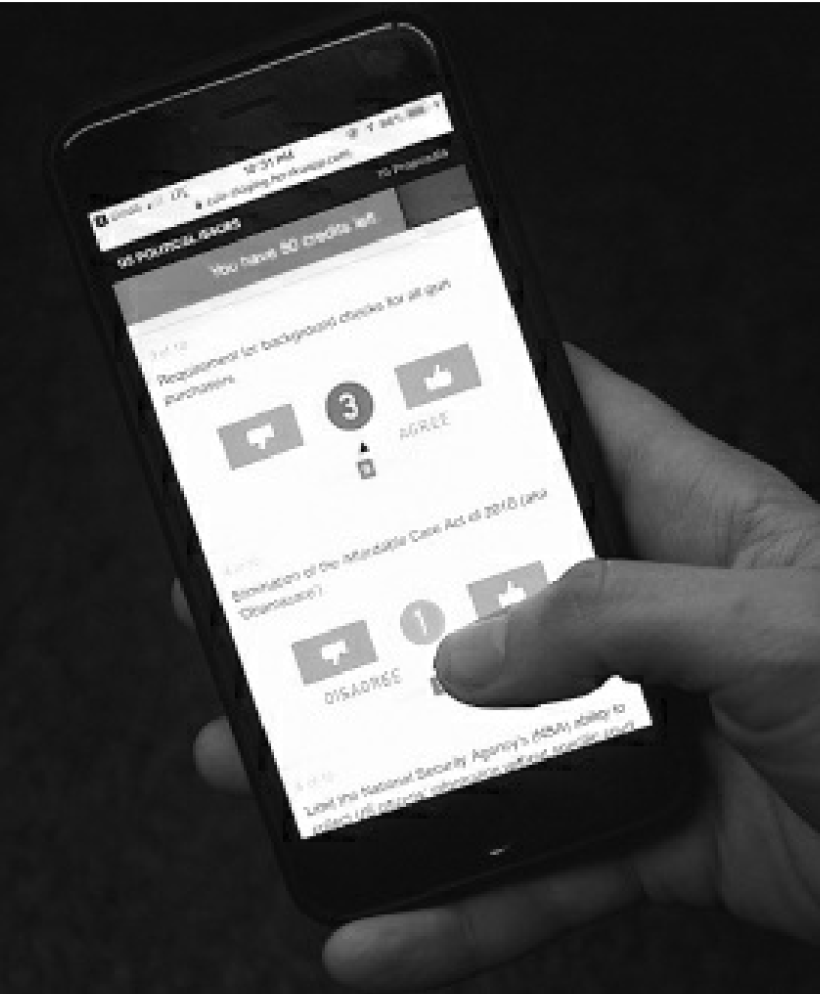
\includegraphics[width=0.4\textwidth]{content/image/curr_interface/radical_market_wedesign.png}
%         \caption{Software by WeDesign, used in the first empirical QV research~\cite{quarfoot2017quadratic}. Little information is available about the software, except for an image from~\textcite{posner2018radical}. In the image, each prompt has thumbs up and down icons to update the vote in the center. The remaining budget appears as a progress bar at the top.}
%         \Description{A black and white image of a mobile phone displaying a voting interface from software by WeDesign, used in empirical QV research. A hand holds the phone, and the screen shows a prompt related to background checks for gun purchases. There are thumbs-up and thumbs-down icons labeled "Agree" and "Disagree," with numbers indicating the current number of votes (e.g., 3 votes for "Agree"). A remaining vote budget is displayed at the top as a progress bar, indicating "50 choices left." The user is interacting with the interface, selecting either agree or disagree on the prompts.}
%         \label{fig:wedesignInterface}
%     \end{subfigure}

%     \vspace{1cm}

%     \begin{subfigure}[b]{1\textwidth}
%         \centering
%         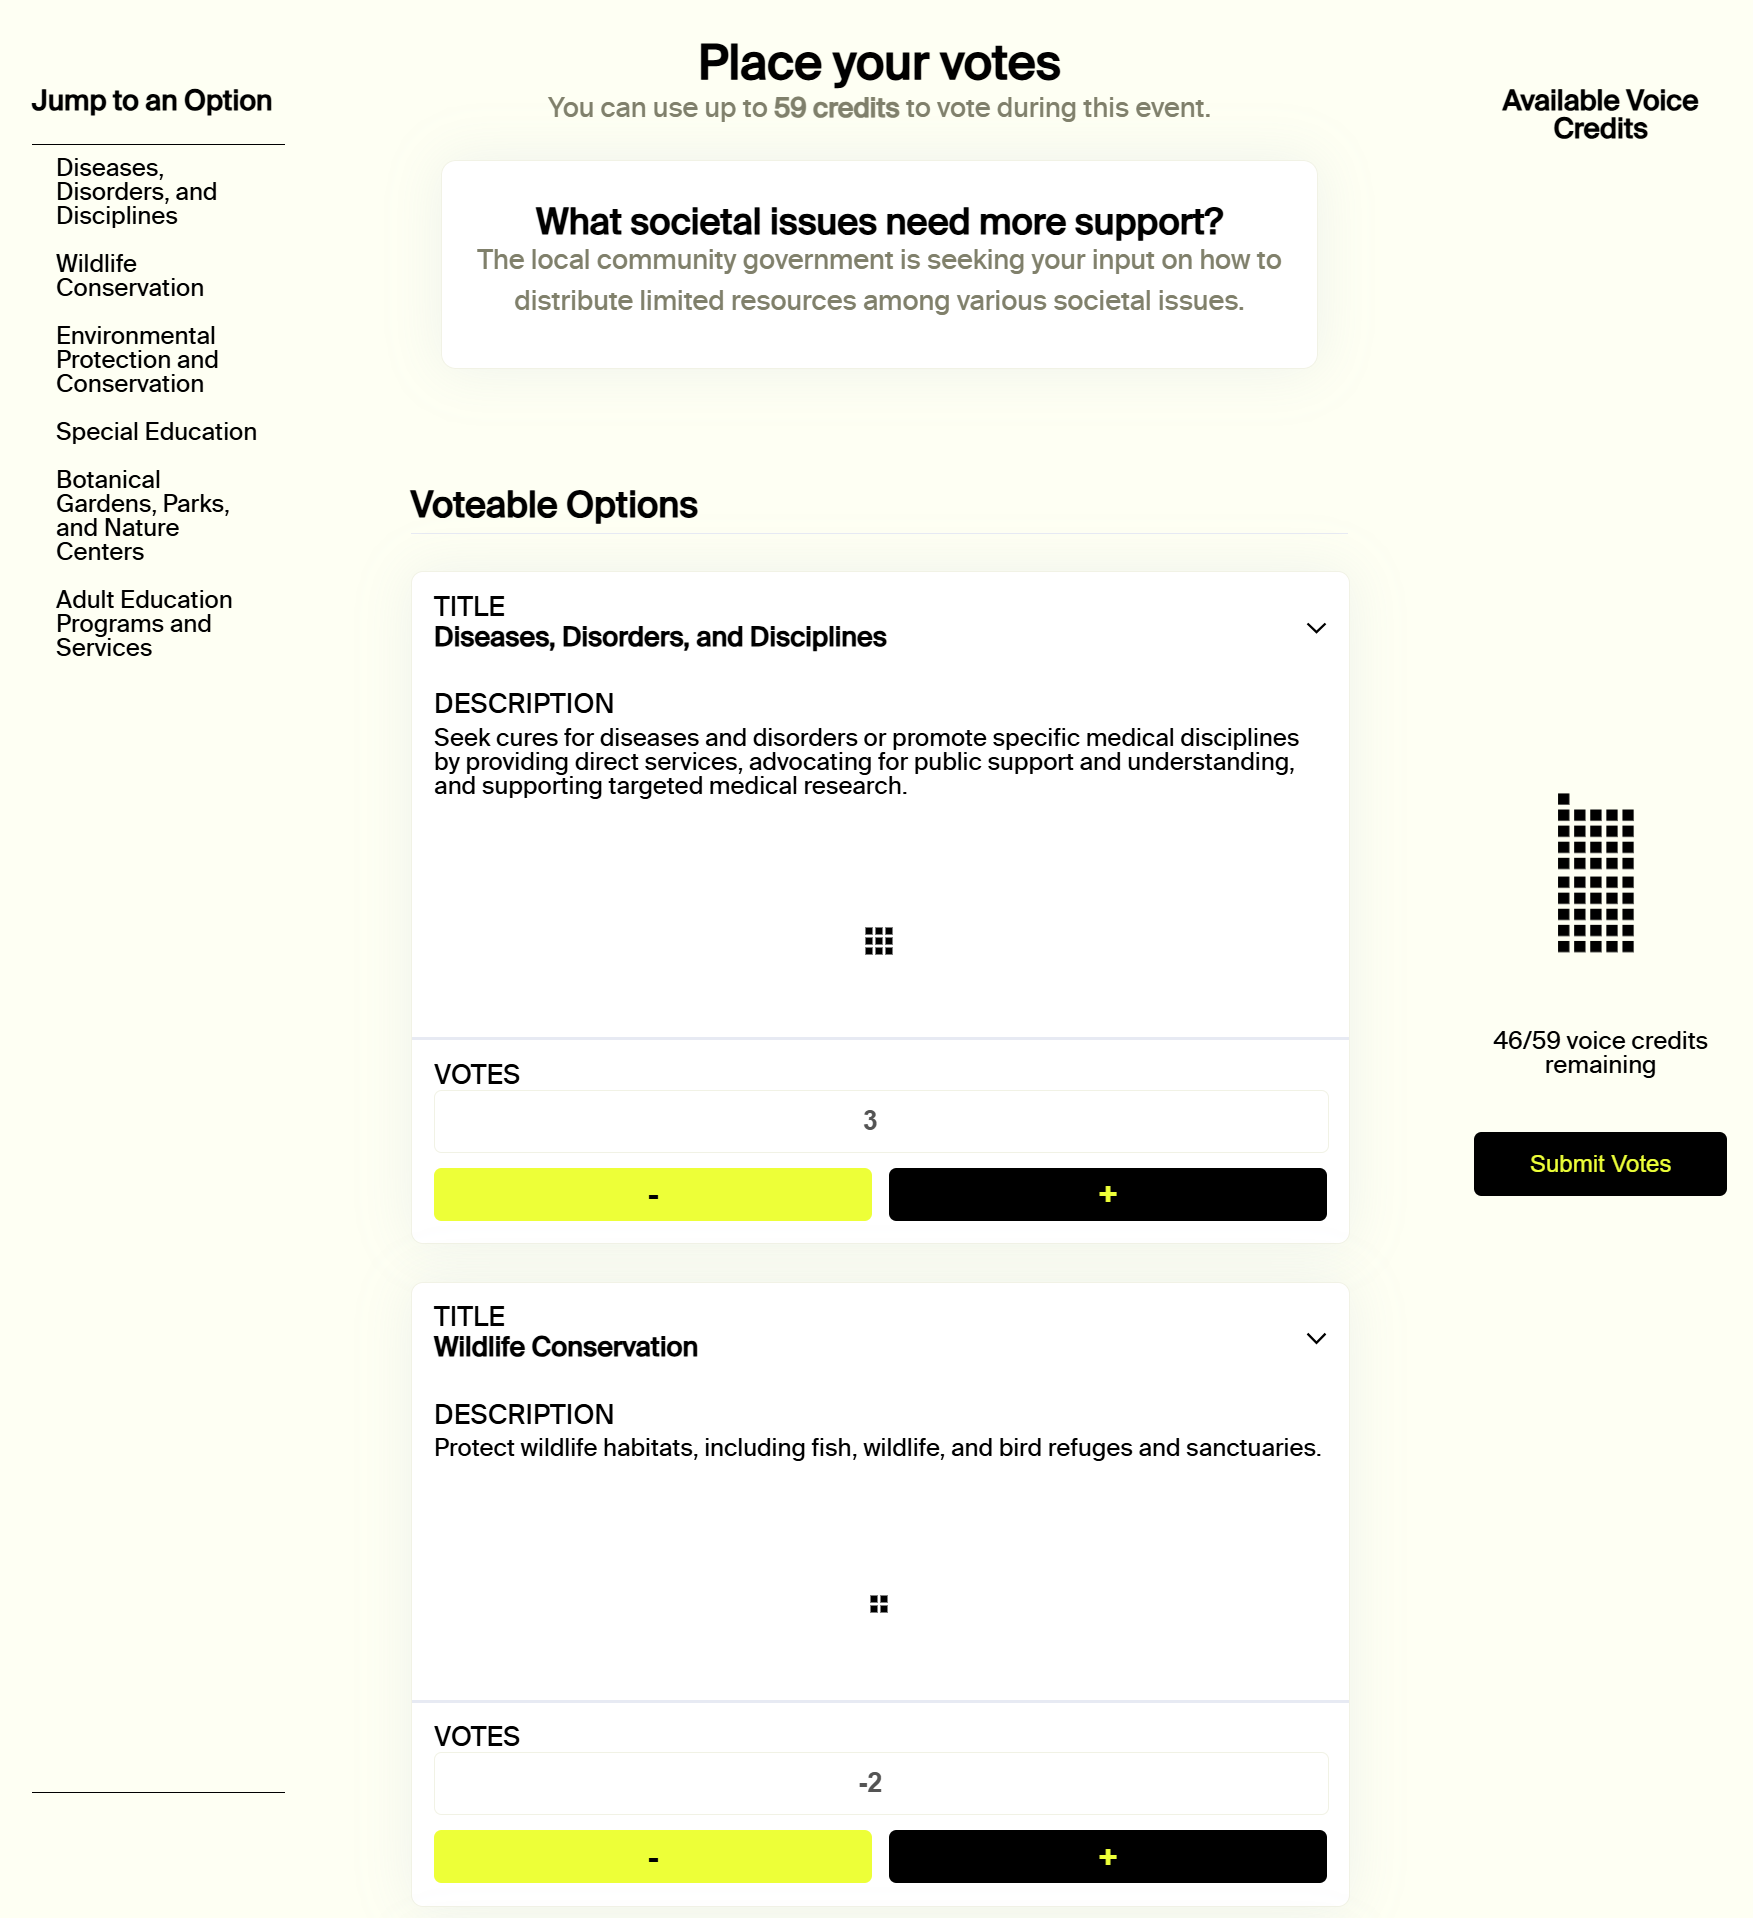
\includegraphics[width=0.5\textwidth]{content/image/curr_interface/rxc_interface.png}
%         \caption{An open-sourced QV interface~\cite{RadicalxChangeQuadraticvoting2024} forked from GitCoin~\cite{ReadWhitepaperGitcoin}, used by the RadicalxChange community~\cite{RxC}. This interface presents total credits as small blocks. Votes are updated using plus and minus buttons, with numerical counts shown under each option and surface area as costs.}
%         \Description{A screenshot of a Quadratic Voting (QV) interface designed for voting on societal issues that need more support. The screen displays two options: "Diseases, Disorders, and Disciplines" and "Wildlife Conservation," with a brief description under each. Users can adjust votes with plus and minus buttons, and the current vote count (e.g., 3 votes for Diseases, -2 votes for Wildlife Conservation) is displayed. The total available credits are shown on the right side as a grid of small blocks, with 46 out of 59 credits remaining. There is also a "Submit Votes" button. A menu on the left allows users to jump to different societal issues.}
%         \label{fig:rxcvotingInterface}
%     \end{subfigure}
    
%     % \vspace{0.12cm}
    
%     % \begin{subfigure}[b]{0.47\textwidth}
%     %     \centering
%     %     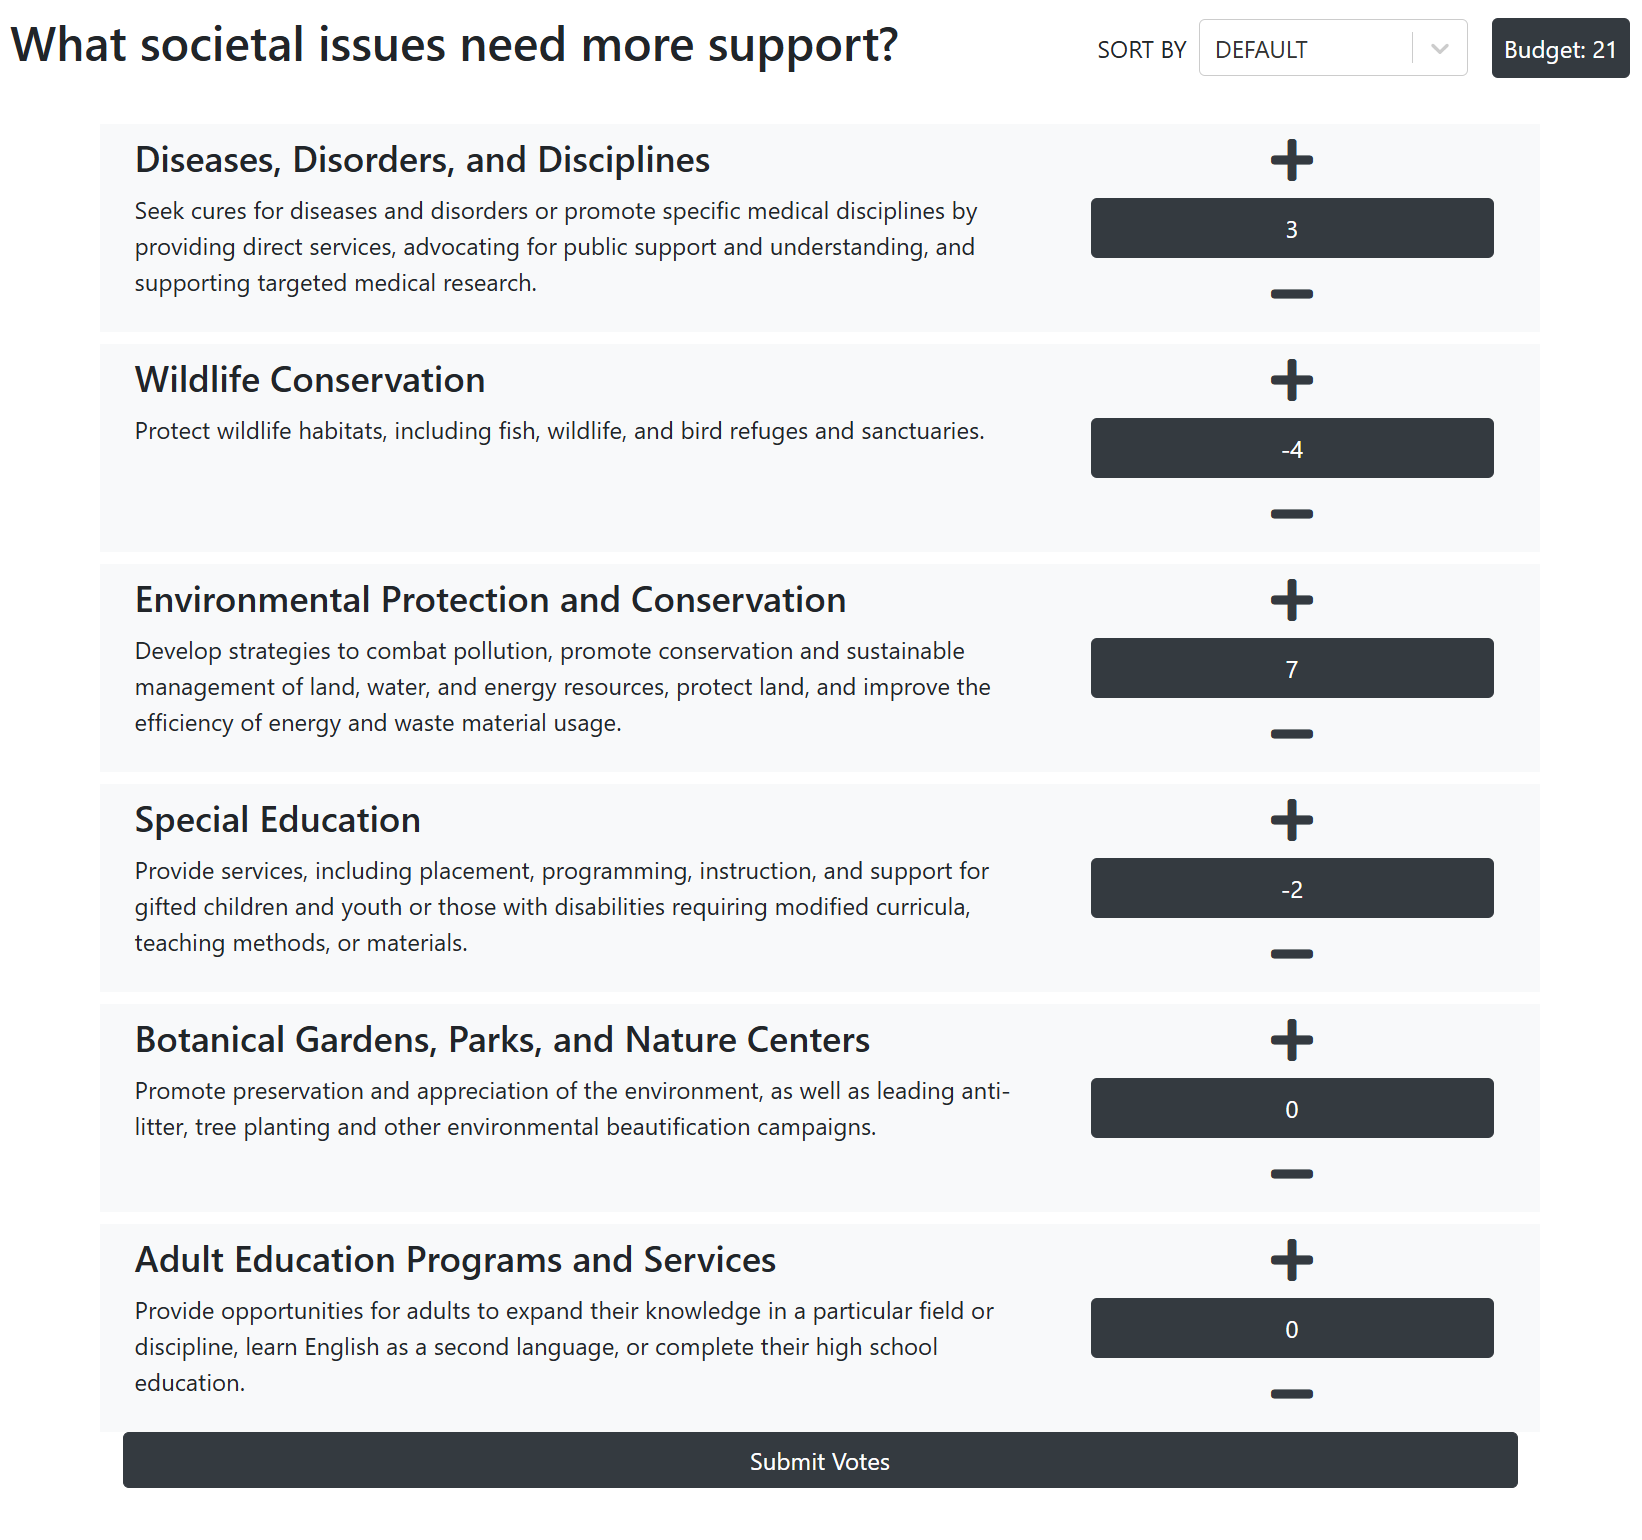
\includegraphics[width=0.72\textwidth]{content/image/curr_interface/geek.sg_interface.png}
%     %     \caption{An open-source QV interface~\cite{yehjxraymondYehjxraymondQvapp2024} offers a publicly available service. Options show only the current number of votes, with credits displayed in the top right corner. This interface does not show the costs of votes but supports sorting options.}
%     %     \Description{A screenshot of a Quadratic Voting (QV) interface for selecting societal issues that need more support. The interface presents six options: "Diseases, Disorders, and Disciplines," "Wildlife Conservation," "Environmental Protection and Conservation," "Special Education," "Botanical Gardens, Parks, and Nature Centers," and "Adult Education Programs and Services." Each option has a plus and minus button for allocating votes, with the current vote count displayed in a black box (e.g., 3 votes for "Diseases, Disorders, and Disciplines," -4 votes for "Wildlife Conservation," and 7 votes for "Environmental Protection and Conservation"). The budget of 21 credits is shown at the top right of the interface, and there is a "Submit Votes" button at the bottom. The interface also includes a sorting option set to "Default," though no vote cost information is displayed.}
%     %     \label{fig:yehInterface}
%     % \end{subfigure}
%     % \hspace{0.4cm}
%     % \begin{subfigure}[b]{0.47\textwidth}
%     %     \centering
%     %     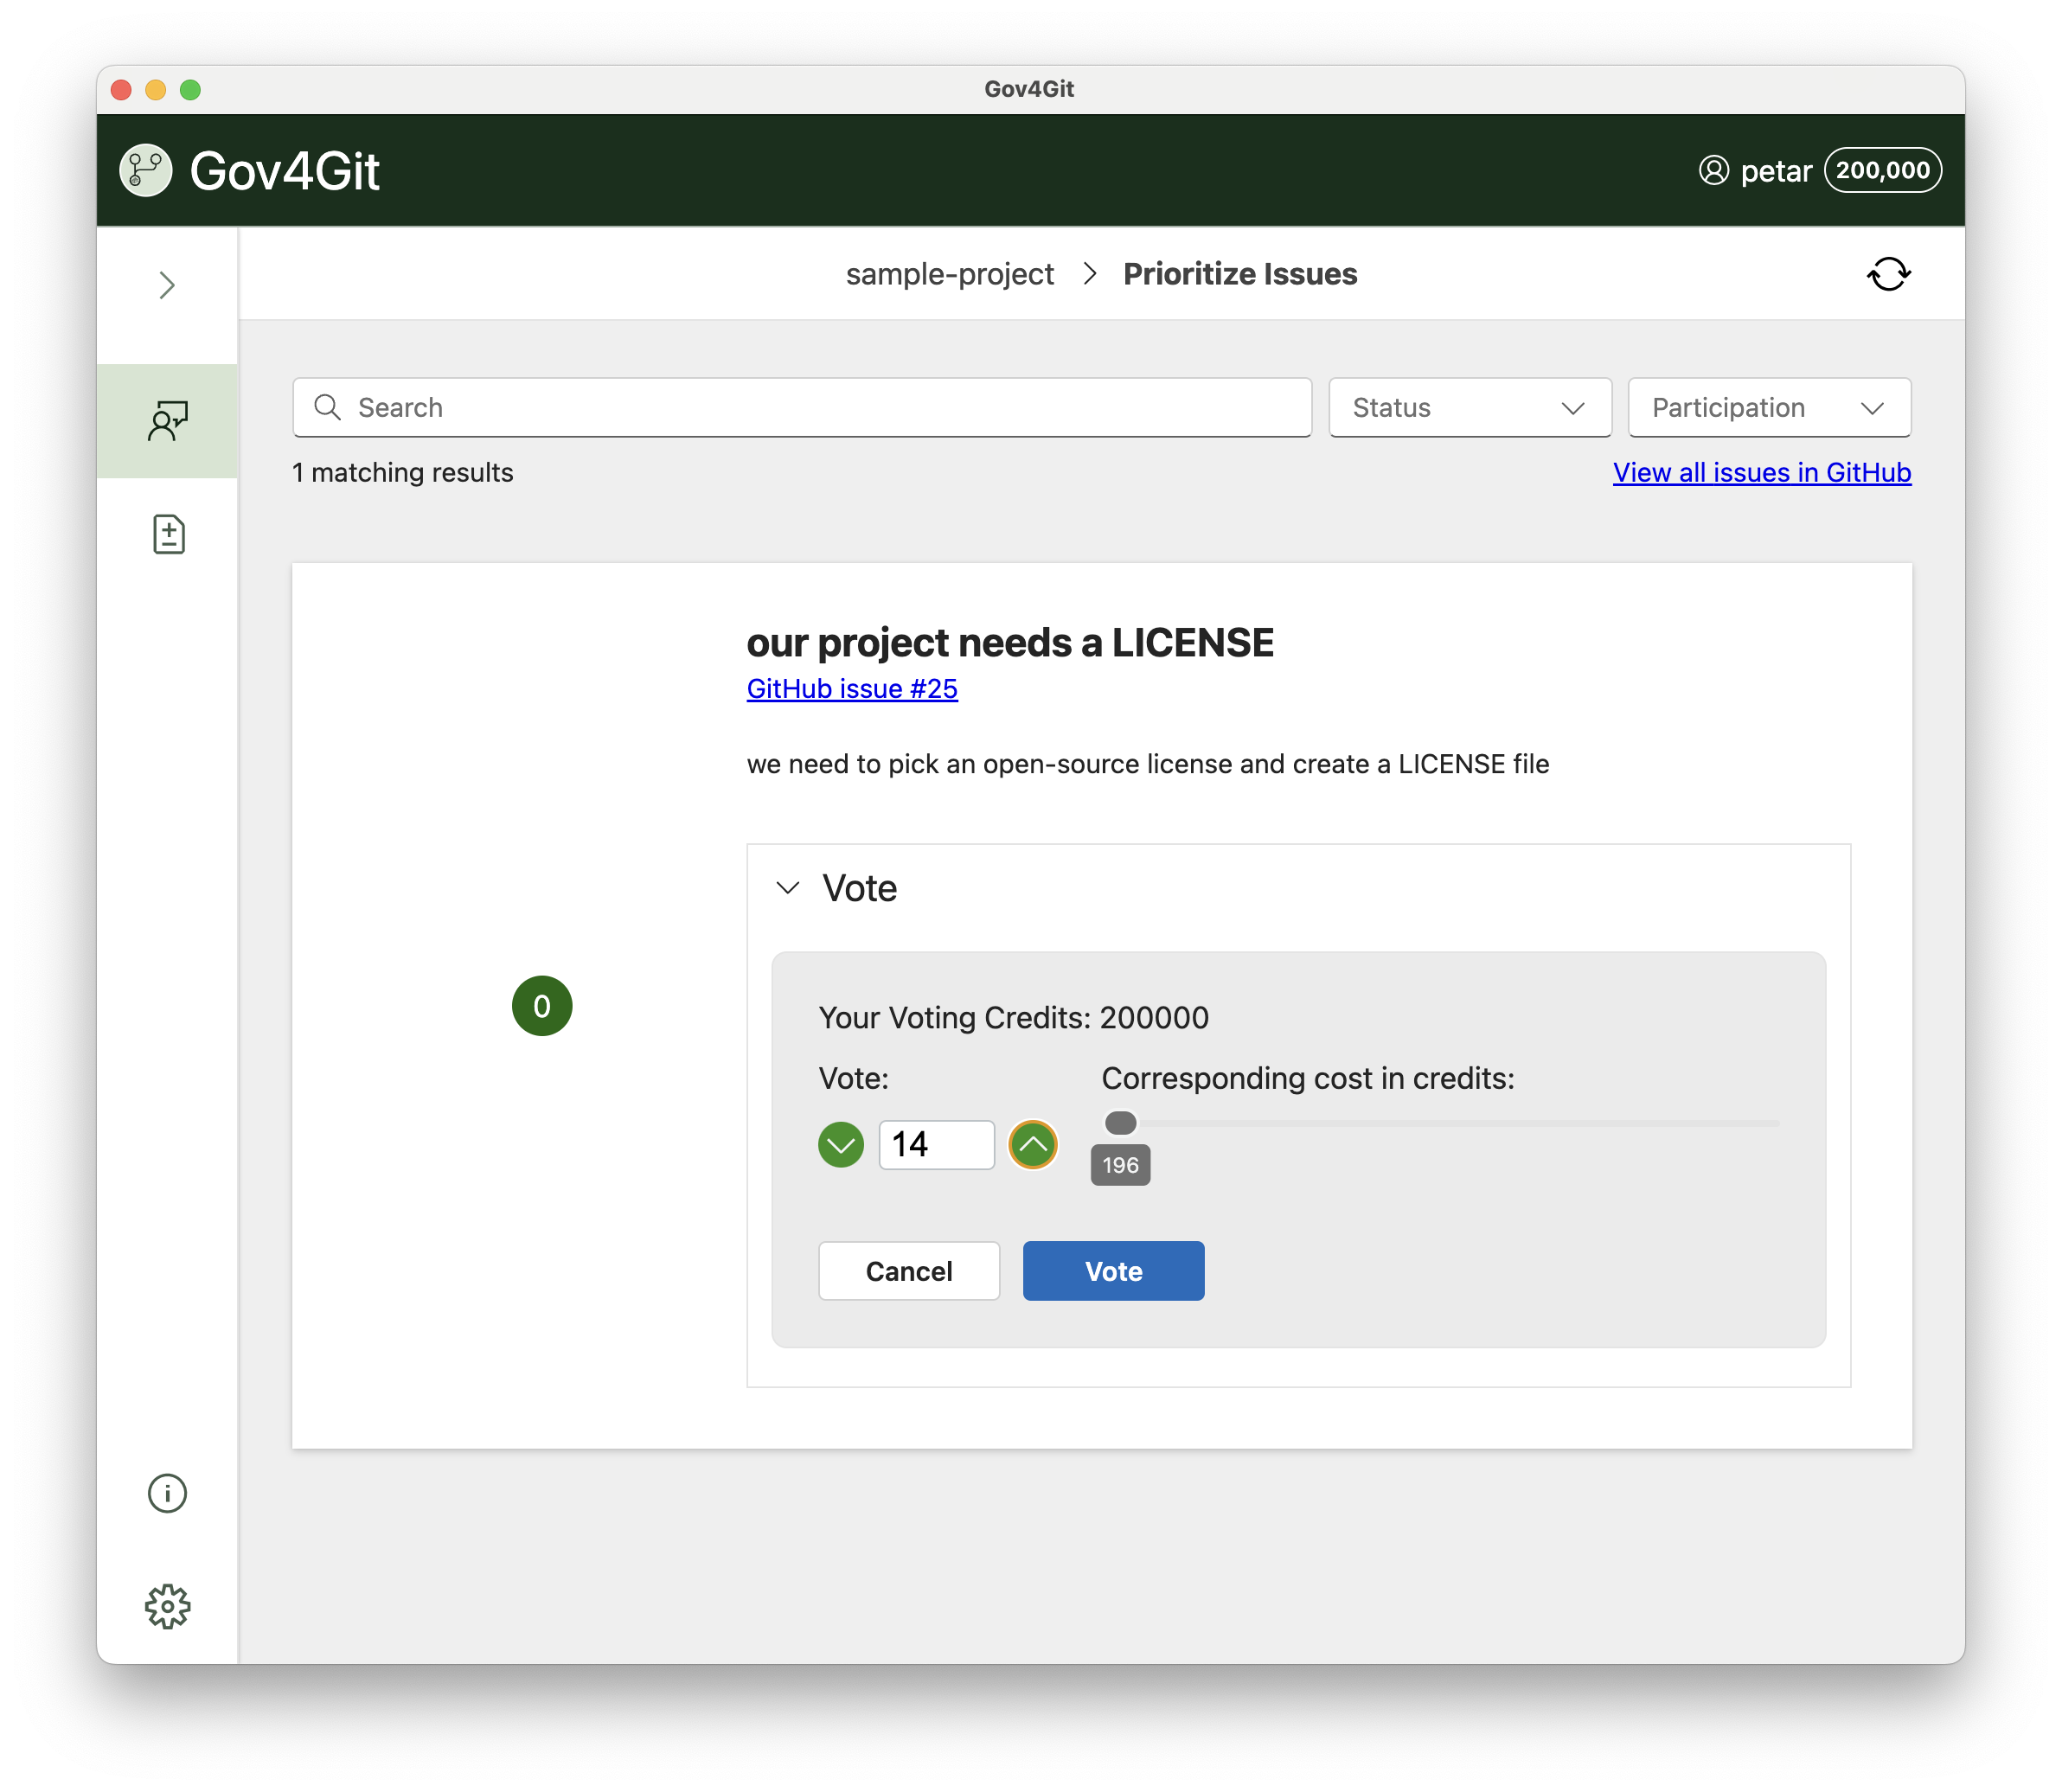
\includegraphics[width=0.72\textwidth]{content/image/curr_interface/appvote.png}
%     %     \caption{The interface designed for gov4git~\cite{Gov4gitDecentralizedPlatform2023} updates votes using arrows under each option, with the associated cost shown as a percentage bar to the right. A search bar exists for searching specific pull requests or issues.}
%     %     \Description{The screenshot displays the interface of the Gov4Git application on a desktop browser. At the top left, the Gov4Git logo and the project name "sample-project" are shown, with a breadcrumb navigation bar leading to "Prioritize Issues." Below, the main section shows an issue titled "our project needs a LICENSE," linked to a corresponding GitHub issue \#25. The text suggests that the team needs to select an open-source license. Below the issue description is a "Vote" box displaying available voting credits (200,000) and options to vote with a green up-arrow. The user has entered a vote of 14, with a corresponding cost of 196 credits shown next to the percentage bar. Options to cancel or submit the vote are shown at the bottom. The interface includes a search bar and drop-down filters for status and participation. The user is identified at the top right as "petar" with 200,000 credits.}
%     %     \label{fig:gov4gitInterface}
%     % \end{subfigure}
    
%     % \vspace{0.15cm}
    
%     % \begin{subfigure}[b]{0.7\textwidth}
%     %     \centering
%     %     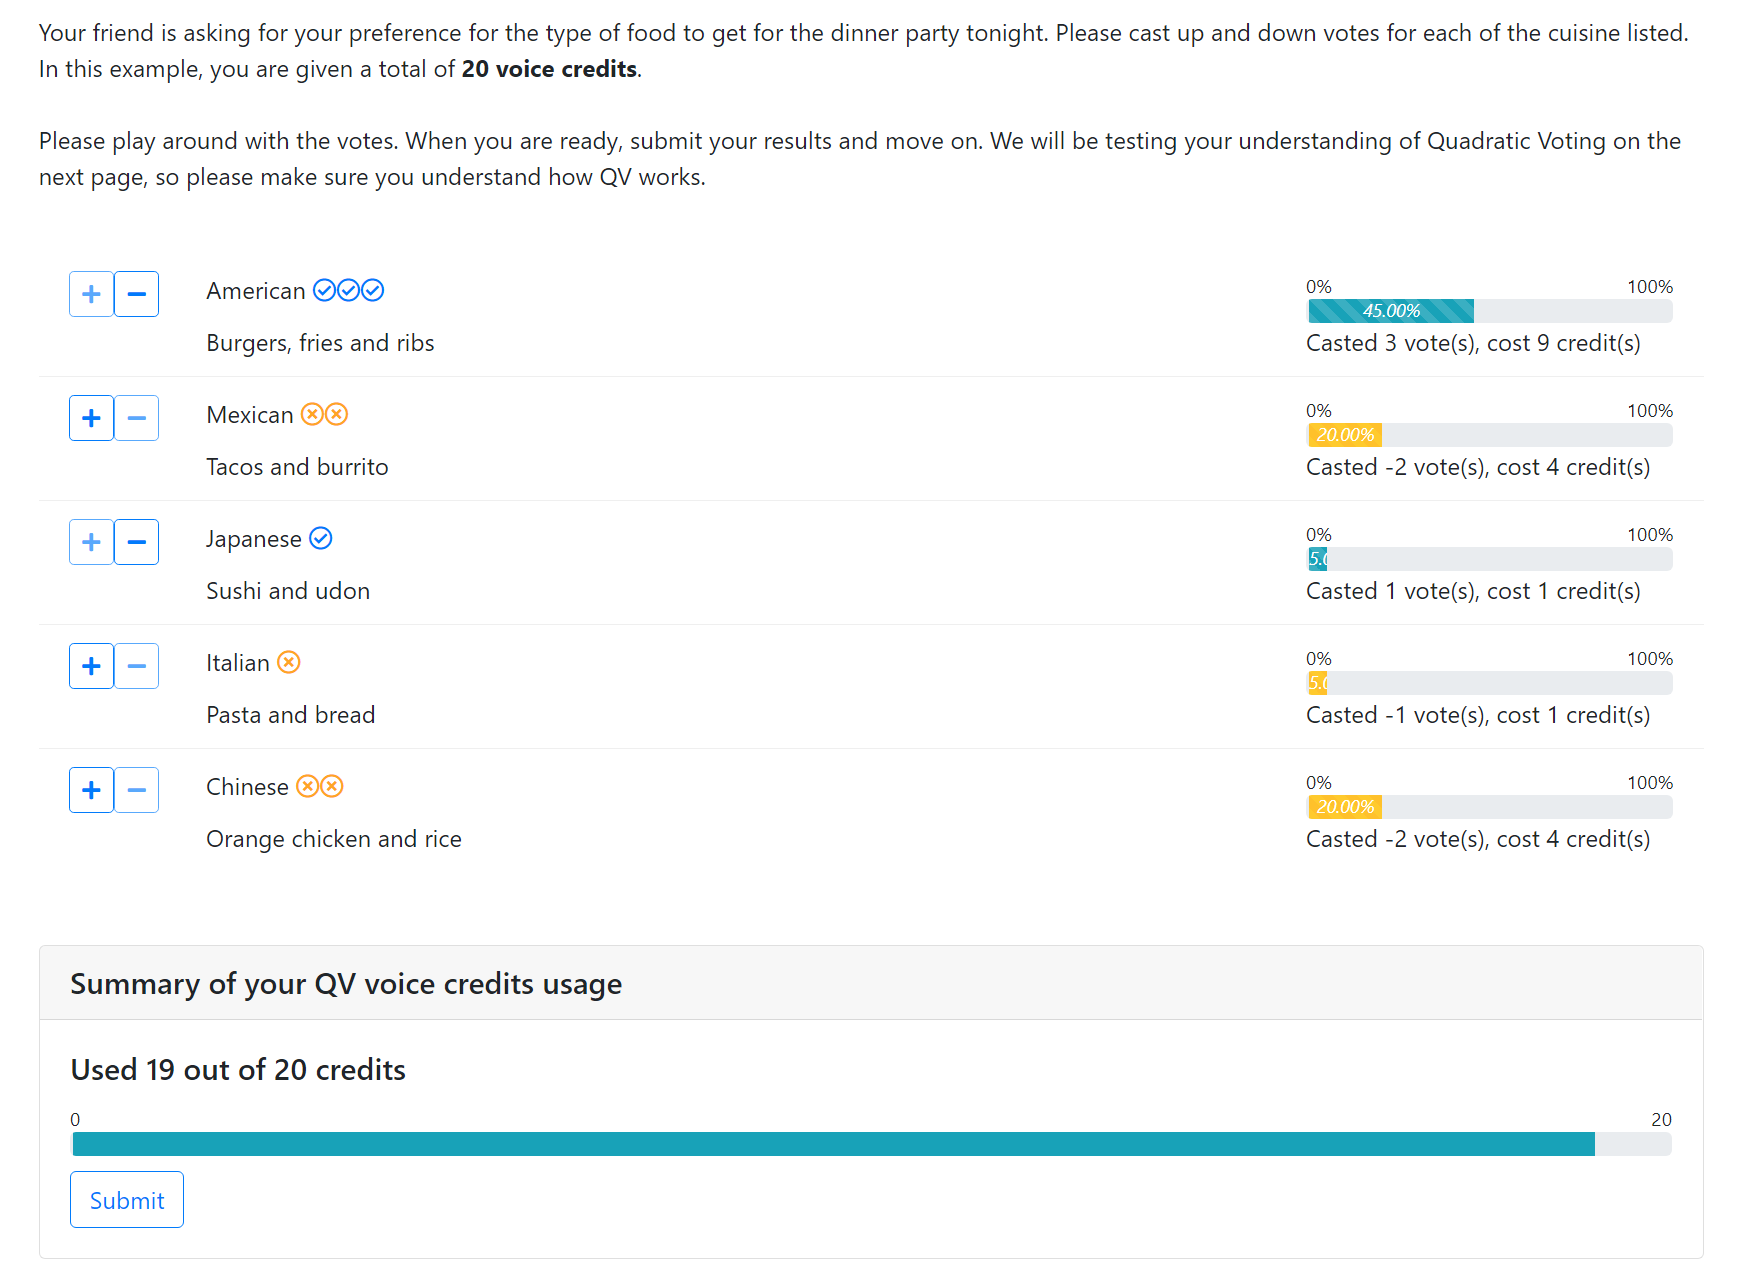
\includegraphics[width=0.50\textwidth]{content/image/curr_interface/cheng_qv.png}
%     %     \caption{The interface used in the research by~\textcite{chengCanShowWhat2021} employs the most visual components. Icons depict the current number of votes, with progress bars signifying the current spending.}
%     %     \Description{A screenshot of a Quadratic Voting (QV) interface, where users are asked to allocate 20 voice credits to vote on preferred food options for a dinner party. The interface presents five cuisine options: American (burgers, fries, and ribs), Mexican (tacos and burritos), Japanese (sushi and udon), Italian (pasta and bread), and Chinese (orange chicken and rice). Each option has plus and minus buttons to increase or decrease votes, along with icons displaying the number of votes placed. A progress bar beside each cuisine shows the percentage of votes cast, and corresponding text details the number of votes and credits used (e.g., 3 votes for American costing 9 credits). Below the voting section, a summary bar shows the total of 19 out of 20 credits used, with a "Submit" button at the bottom of the page.}
%     %     \label{fig:chengInterface}
%     % \end{subfigure}
    
%     \caption{Recent interface for applications using the quadratic mechanism.}
%     \Description{A collection of 5 interfaces showcasing various interfaces.}
%     \label{fig:qv_interface_external}
% \end{figure}
% \clearpage
% }
\begin{figure}[h]
    \centering
    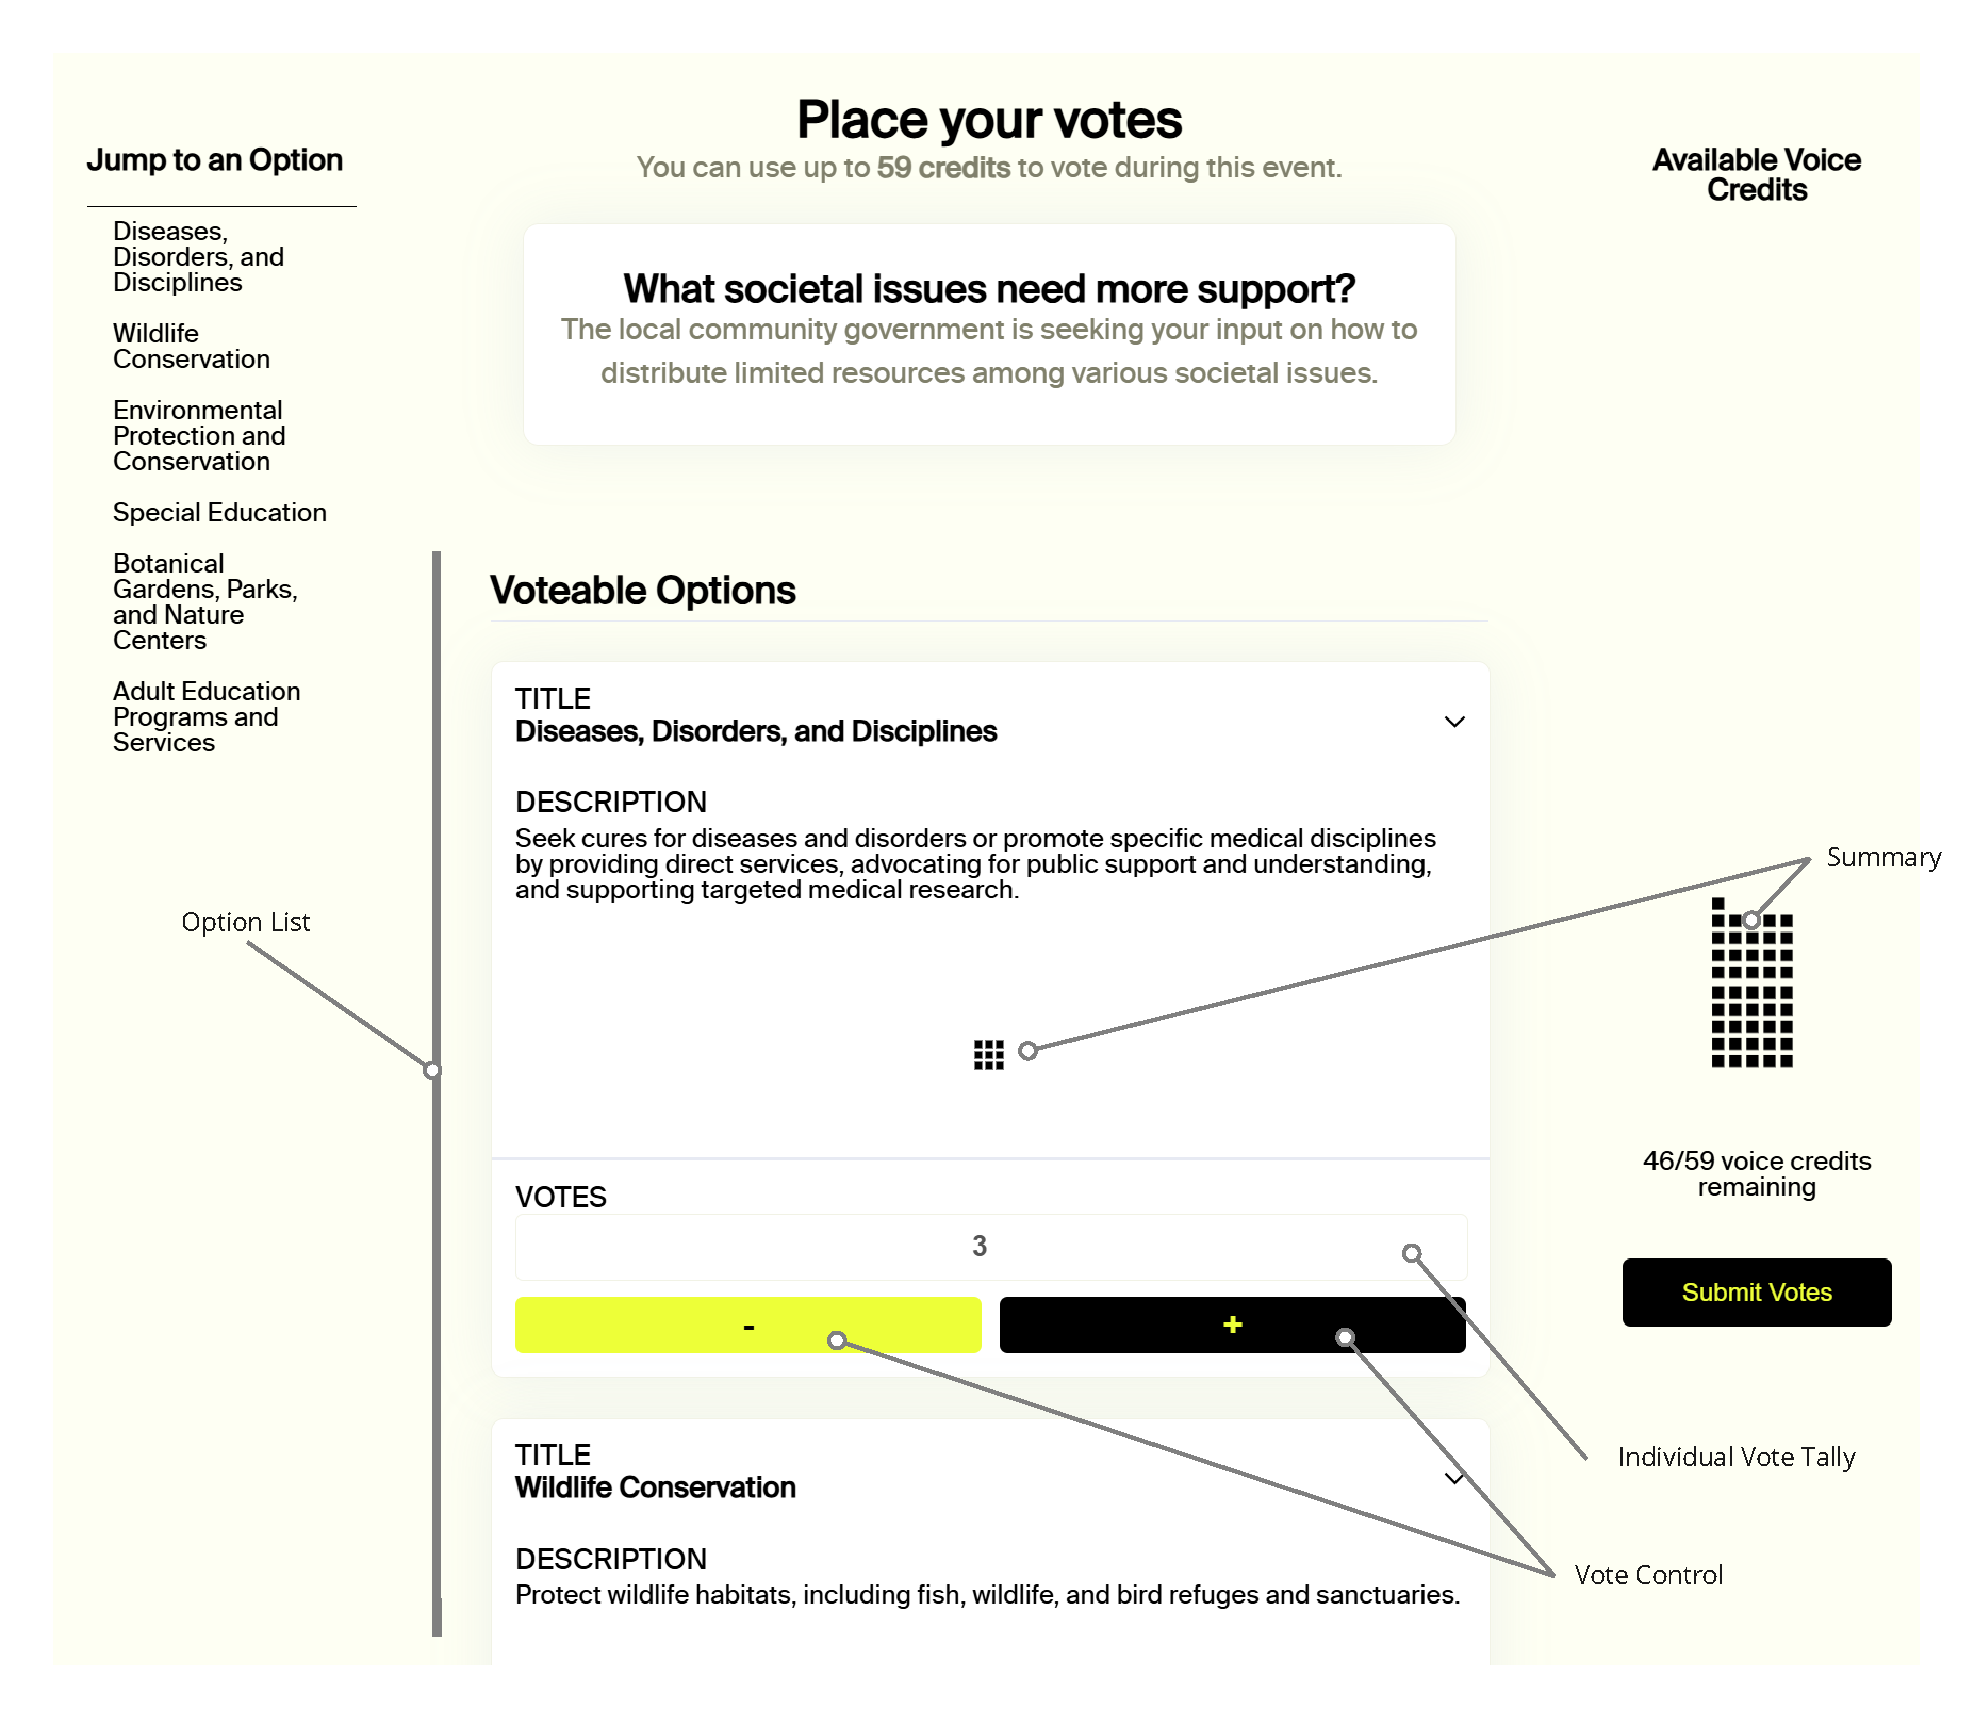
\includegraphics[width=0.7\textwidth]{content/image/curr_interface/rxc_interface_annotated.pdf}
    \caption{An open-sourced QV interface~\cite{RadicalxChangeQuadraticvoting2024} forked from GitCoin~\cite{ReadWhitepaperGitcoin}, used by the RadicalxChange community~\cite{RxC}. Votes are updated through plus and minus buttons, with numerical vote tallying under each option. This interface used small blocks to represent remaining credits and individual option costs.}
    \Description{}
    \label{fig:rcx_interface_annotated}
\end{figure}

\begin{figure}[h]
    \centering
    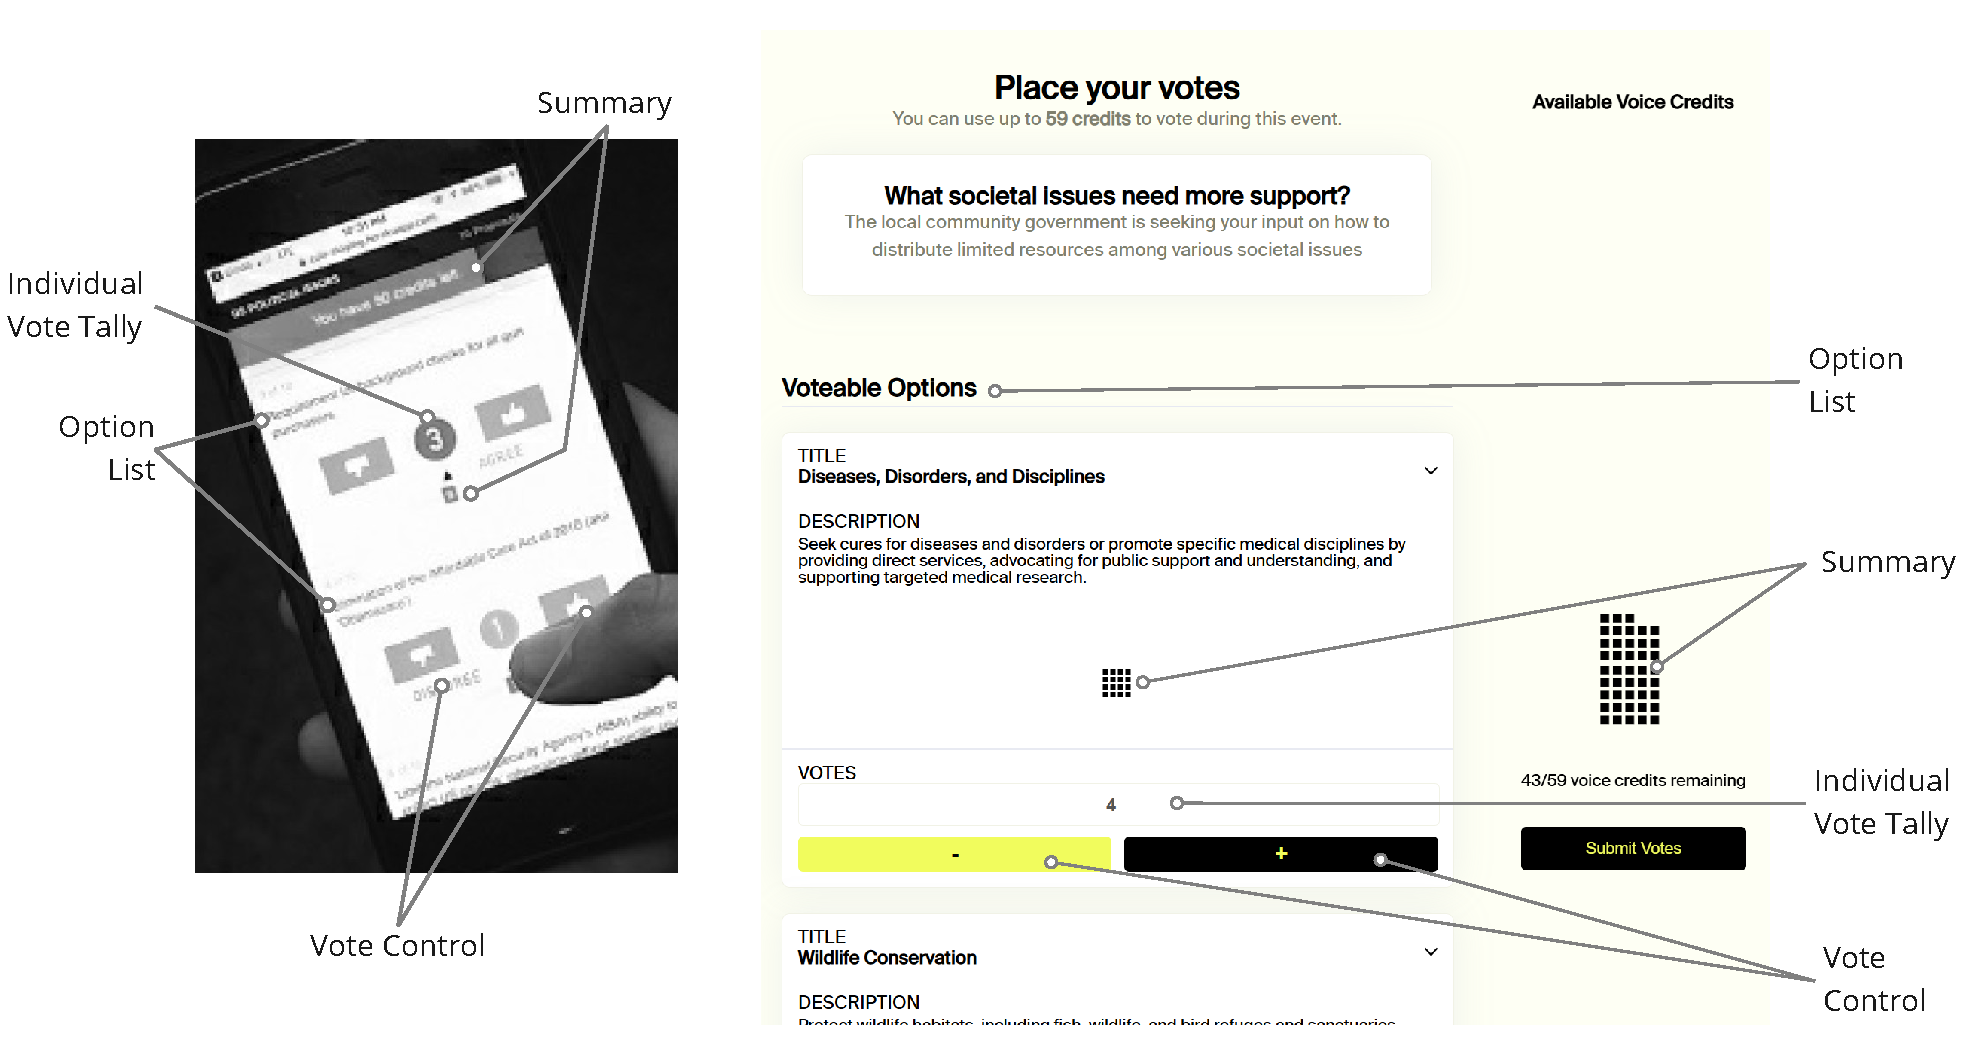
\includegraphics[width=\textwidth]{content/image/curr_interface/recent_annotated.pdf}
    \caption{An open-sourced QV interface~\cite{RadicalxChangeQuadraticvoting2024} forked from GitCoin~\cite{ReadWhitepaperGitcoin}, used by the RadicalxChange community~\cite{RxC}. Votes are updated through plus and minus buttons, with numerical vote tallying under each option. This interface used small blocks to represent remaining credits and individual option costs.}
    \Description{}
    \label{fig:rcx_interface_annotated}
\end{figure}

%     \begin{subfigure}[b]{1\textwidth}
%         \centering
%         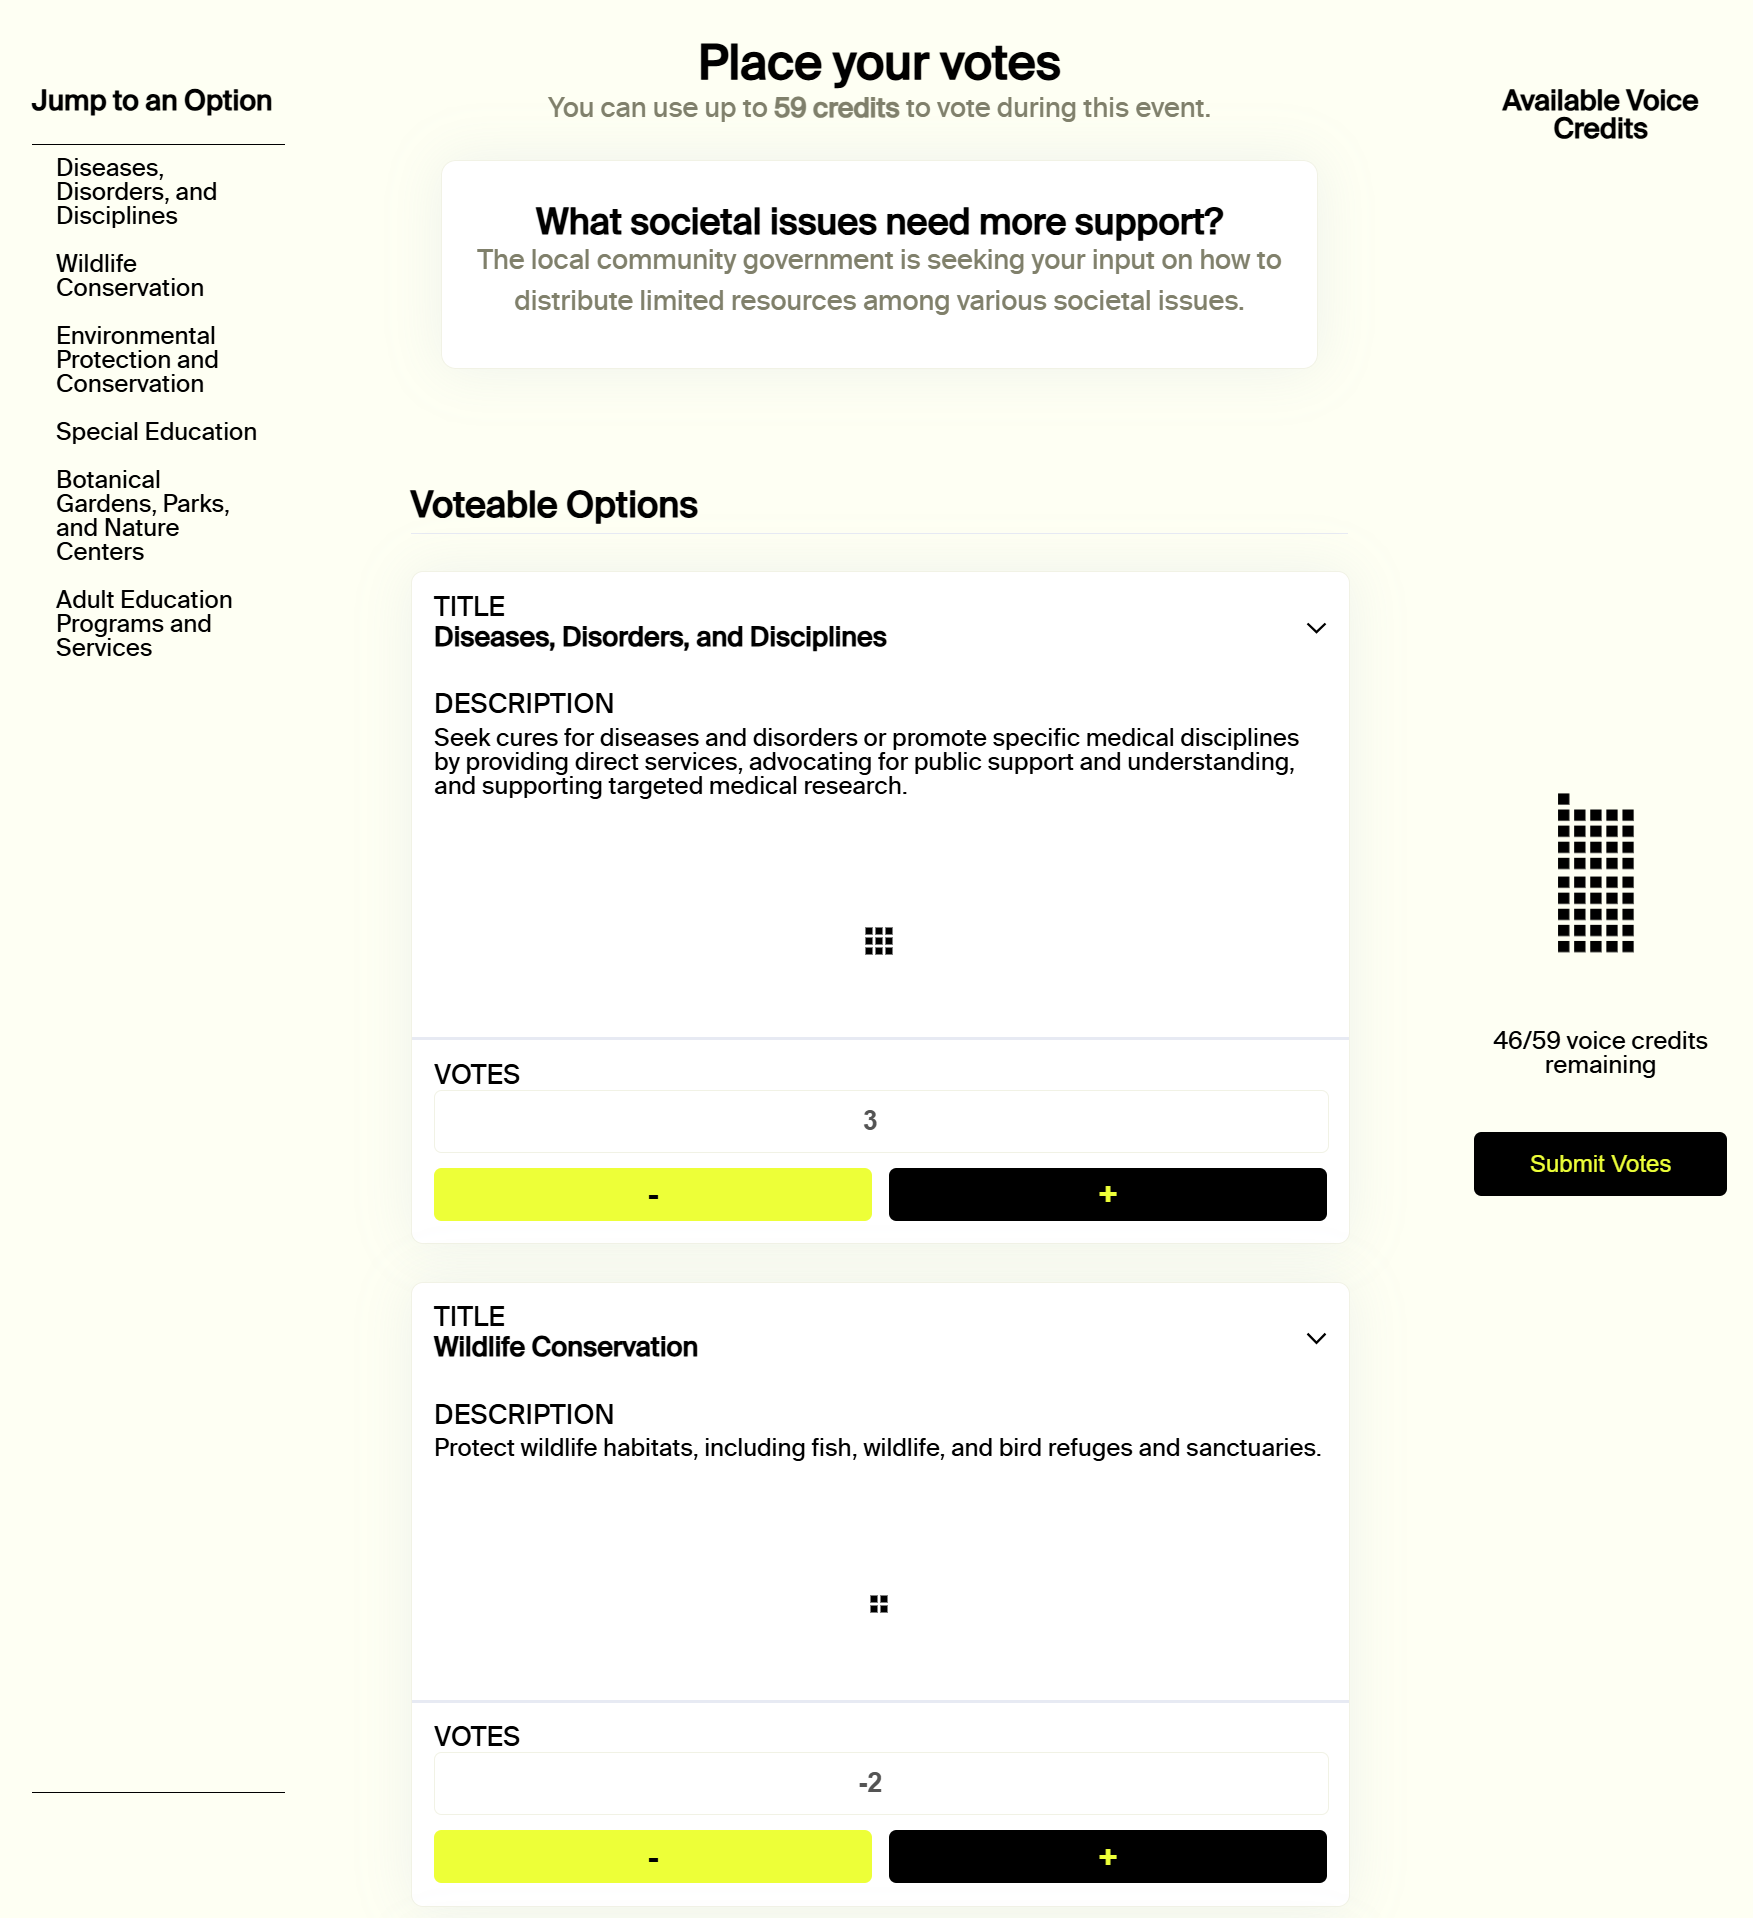
\includegraphics[width=0.5\textwidth]{content/image/curr_interface/rxc_interface.png}
%         \caption{An open-sourced QV interface~\cite{RadicalxChangeQuadraticvoting2024} forked from GitCoin~\cite{ReadWhitepaperGitcoin}, used by the RadicalxChange community~\cite{RxC}. This interface presents total credits as small blocks. Votes are updated using plus and minus buttons, with numerical counts shown under each option and surface area as costs.}
%         \Description{A screenshot of a Quadratic Voting (QV) interface designed for voting on societal issues that need more support. The screen displays two options: "Diseases, Disorders, and Disciplines" and "Wildlife Conservation," with a brief description under each. Users can adjust votes with plus and minus buttons, and the current vote count (e.g., 3 votes for Diseases, -2 votes for Wildlife Conservation) is displayed. The total available credits are shown on the right side as a grid of small blocks, with 46 out of 59 credits remaining. There is also a "Submit Votes" button. A menu on the left allows users to jump to different societal issues.}


\change{
\subsection{Design Implications existing QV Interfaces}
\change{Given QS shares the same mechanism with QV, we conducted a snowball sampling process to identify publicly available Quadratic Voting (QV) applications from known news reports and academic publications. No widely adopted QV interfaces have been developed by a single vendor or platform to date. Fig.~\ref{fig:rcx_interface_annotated} shows two variations of existing interfaces~\footnote{Appendix X lists a comprehensive list we surveyed}, with all QV interfaces employing a single-step approach with different visual representations of common elements.} All QV interfaces generally include:

\begin{itemize}
    \item Option list: A list of options for voting.
    \item Vote controls: Buttons to increase or decrease votes for each option.
    \item Individual vote tally: A display of the votes cast per option.
    \item Summary: An auto-generated summary of costs and the remaining budget.
\end{itemize}

\change{These components allow individuals to operate QV, focusing purely on mechanics without little understanding of voters' usability needs nor offering cognitive support to help them complete the task.} In addition, the HCI community conducted few research~\cite{nobarany2012design, van2007design} on survey and questionnaire interfaces components, with more work focusing more on alternative input modalities like bots, voice, and virtual reality~\cite{voiceWei2022, khullar2021, kimComparingDataChatbot2019, feick2020virtual}.}

\subsection{Cognitive Challenges and Choice Overload}
The challenge of respondents making difficult decisions using quadratic mechanisms remains unexplored in the literature.~\textcite{lichtensteinConstructionPreference2006} identified three key elements that make decisions difficult. \change{These elements include making decisions in unfamiliar contexts, quantifying the value of one's opinions, and being forced to make trade-offs due to conflicting choices. QS fits at least two of the three elements: participants may encounter a selection of unfamiliar options by the survey designer; they are asked to quantify the difference between option preferences through a numerical vote; and the budget constraint enforces trade-offs under a non-linear function, which means that a vote decrease for one option is not necessary equivalent to an increase for another, making iterative adjustment and evaluating tradeoffs difficult. Thus, we believe QS introduces a high cognitive load.}

Cognitive load refers to the demands placed on a user's working memory during the interaction process, which significantly influences the usability of the system~\cite{cooper1998research, seppCognitiveLoadTheory2019}. Cognitive overload can adversely affect performance~\cite{drommi2001interface}, leading individuals to rely on heuristics rather than deliberate, logical decision-making~\cite{daniel2017thinking}. When presented with excessive information, such as too many options, individuals 'satisfice', settling for a 'good enough' solution rather than an optimal one~\cite{simonBehavioralModelRational1955, payneAdaptiveStrategySelection1988, tverskyJudgmentsRepresentativeness}. Subsequently, too many options can overwhelm individuals, resulting in decision paralysis, demotivation, and dissatisfaction~\cite{iyengarWhenChoiceDemotivating2000}.

Additionally,~\textcite{alwinMeasurementValuesSurveys1985} highlighted that the use of ranking techniques in surveys can be time-consuming and potentially more costly to administer. These challenges are compounded when ranking numerous items, requiring substantial cognitive sophistication and concentration from survey respondents \cite{featherMeasurementValuesEffects1973}.

Notable applications of Quadratic Voting include the $2019$ Colorado House, which considered $107$ bills~\cite{coyNewWayVoting2019}, and the $2019$ Taiwan Presidential Hackathon, which featured $136$ proposals~\cite{QuadraticVotingFrontend2022}; both used a single QV question with hundreds of options.~\change{These empirical applications of QV suggest the importance of understanding QS with many options' impact on cognitive load and support developing interfaces for practical uses.}

% Psychological and behavioral research highlights the importance of understanding how individuals navigate and benefit from new interfaces under long-list QS conditions. These empirical applications of QV suggest QS's potential to elicit individual preferences, emphasizing the need to study cognitive load and interface design.

%  Removed text and citations
% These influences can even increase dropouts due to additional burdens on survey respondents~\textcite{galesicDropoutsWebEffects2006} which reduces the urge for researchers to use QS.
%As \textcite{chengCanShowWhat2021} noted, it is essential to better understand how the number of options influences the usability of QS and to design interfaces that effectively support survey respondents.
% there is limited research on interfaces for Constant Sum surveys~\cite{hauserIntensityMeasuresConsumer1980a}, a mechanism similar to QS that aims to elicit both ranking and rating preferences from individuals.
%The closest work discussing interfaces for QV is an arXiv paper~\cite{} that transformed the knapsack voting platform developed by \textcite{goelKnapsackVotingVoting}
% While both fields have deep insights into understanding design's influence on attitude elicitation, QS's unique capability of supporting both ranking and rating~\cite{chengCanShowWhat2021} makes designing an interface important and challenging. Subsequently, this research aims to understand how this interface influences an individual's QS response behavior. Requiring the distribution of budgets following the quadratic mechanism introduces new and complex decisions. 
% Empirical studies and applications of the quadratic mechanism and quadratic voting have increased in the past few years. Several studies have explored the empirical use cases for QV, including \textcite{quarfoot2017quadratic}'s study on 4,500 participants' attitudes across ten public policies, highlighting differences between QV and Likert scale survey results. \textcite{chengCanShowWhat2021} applied quadratic surveys in Human-Computer Interaction (HCI) and subsequently showed QV's effectiveness in reflecting true preferences in monetary decision tasks. \textcite{naylor2017first} used QV in educational research to gauge student opinions on factors affecting university success, and \textcite{cavailleWhoCaresMeasuring} examined QV in polarized choice scenarios.